%==============================================================================
% Sjabloon poster bachproef
%==============================================================================
% Gebaseerd op document class `a0poster' door Gerlinde Kettl en Matthias Weiser
% Aangepast voor gebruik aan HOGENT door Jens Buysse en Bert Van Vreckem

\documentclass[a0,portrait]{hogent-poster}

\course{Bachelorproef}
\studyprogramme{toegepaste informatica}
\academicyear{2024-2025}
\institution{Hogeschool Gent, Valentin Vaerwyckweg 1, 9000 Gent}

\title{Versterking van bedrijfsnetwerkbeveiliging met behulp van firewall toepassingen binnen VPK Packaging Group.}
\author{Goran Van Damme}
\email{goran.vandamme@student.hogent.be}
\supervisor{Sofie Lambert}
\cosupervisor{Jan Khan (VPK Packaging Group)}

\specialisation{Systeem- en Netwerkbeheer}
\keywords{Bedrijfsnetwerkbeveiliging, firewalltoepassingen, ICS-bescherming, cybersecurity, netwerksegmentatie, toegangscontrole, VPK Packaging Group, productiebedrijf }
\projectrepo{https://github.com/goranvdamme123/BachelorproefGoranVanDamme}

\begin{document}

\maketitle

\begin{abstract}
Door de toename van cyberaanvallen is het voor productiebedrijven zoals VPK Packaging Group cruciaal om hun netwerken beter te beveiligen. Vooral Industrial Control Systems, die vaak draaien op verouderde technologieën, zijn kwetsbaar. Deze bachelorproef onderzoekt of de huidige firewalloplossing op de VPK-site in Alizay, waar een Sophos firewall actief is, volstaat of dat een overstap naar de Palo Alto firewalls die reeds in gebruik zijn op andere VPK sites een betere keuze zijn. Het doel is om systeembeheerders bij VPK te ondersteunen bij het maken van een doordachte firewallkeuze die de continuïteit van de productie waarborgt.

De aanpak bestaat uit literatuuronderzoek, analyses van beide firewallopstellingen en best practices voor het opstellen van een firewall binnen een VPK productiesite. De paper bespreekt de theoretische achtergrond, vergelijkt beide oplossingen en evalueert hun toepasbaarheid binnen de context van VPK.

Uit het onderzoek blijkt dat een overstap naar Palo Alto op termijn de beste optie is, dankzij betere beveiliging, beheerbaarheid en uniformiteit binnen het VPK-netwerk. Dit vraagt wel om een gefaseerde implementatie om productie-onderbrekingen te vermijden.
\end{abstract}

\begin{multicols}{2}

\section{Introductie}
VPK Packaging Group is een producent van duurzame papier en karton verpakkingen. Ze zijn wereldwijd actief in meer dan 70 plants waar in totaal meer dan 7000 mensen te werk gesteld zijn. In 2021 heeft VPK Packaging Group een productiesite voor gerecycleerd papier en karton in Alizay overgenomen, gelegen in Normandië, ten westen van Parijs. Deze site maakt gebruik van een Sophos firewall ter bescherming van het OT netwerk tegen externe dreigingen. Op alle andere VPK-productiesites wordt echter een Palo Alto firewall gebruikt voor de beveiliging van het ICS. Het is dan ook logisch dat de vraag rijst of het behoud van de Sophos firewall op deze locatie effectief en haalbaar is, of dat een vervanging door een Palo Alto firewall die in lijn is met de rest van de VPK sites een betere optie is.

Verder zal dit onderzoek zich richten op de evaluatie van de huidige Sophos firewall op de VPK site in Alizay en onderzoekt in welke mate deze bijdraagt aan de beveiliging van het IT/OT netwerk.
\newline

\begin{center}
    \captionsetup{type=figure}
    \fbox{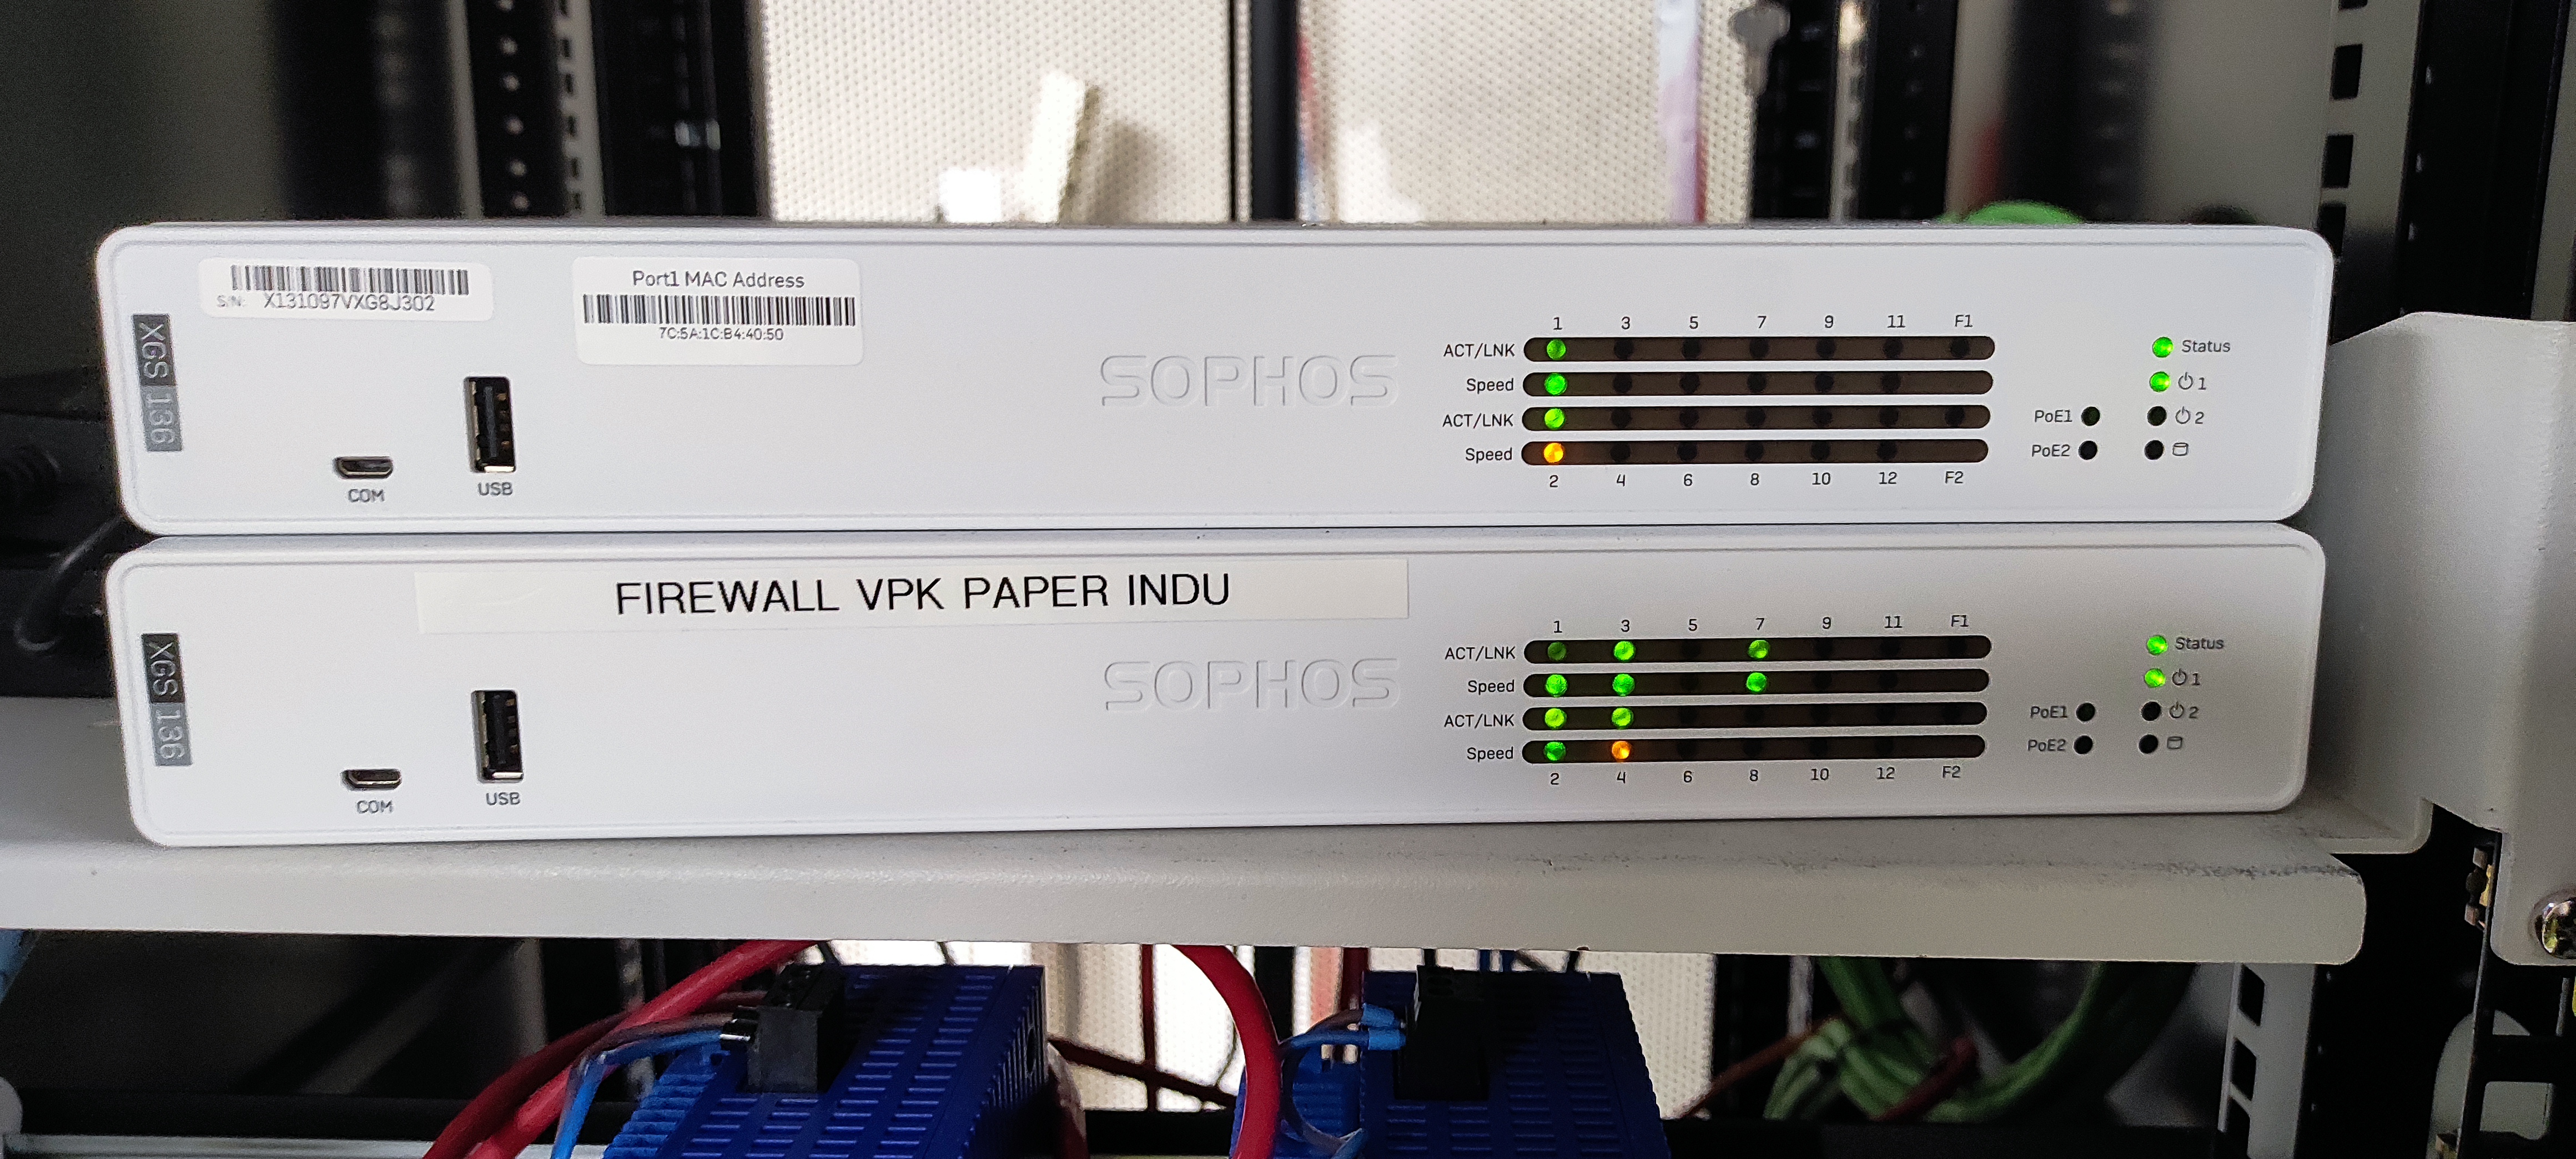
\includegraphics[width=0.46\textwidth]{graphics/SophosFirewall.jpg}}
    \captionof{figure}{De huidige Sophos firewall die gebruikt wordt in de Alizay site van VPK.}
\end{center}


\section{Analyses}
Voor deze studie zijn verschillende analyses uitgevoerd binnen de site van Alizay. De RASCI-analyse brengt de huidige verantwoordelijkheden van de diverse stakeholders binnen het netwerk in kaart. Dit zorgt voor een beter overzicht van wie welke taken uitvoert. Daarnaast is er een geoptimaliseerde RASCI-tabel opgesteld, waarin de rolverdeling efficiënter is ingericht. Hierdoor kunnen taken vlotter en effectiever worden uitgevoerd. Ook is een SWOT analyse uitgevoerd. Deze analyse brengt de sterktes, zwaktes, kansen en bedreigingen van het netwerk duidelijk in beeld en biedt inzicht in de belangrijkste voordelen en aandachtspunten binnen het huidige functioneren van het netwerk.

\section{Configuraties}

Hoe effectief een firewall werkt hangt vaak af van de configuratie die gebeurd is op het apparaat. Daarom is er binnen deze studie ook gekeken naar de verschillende settings die kunnen worden aangepast op de Sophos en de Palo Alto firewall om het ICS netwerk optimaal te beschermen, en waarbij er ook oog is voor de performantie van de firewalls en de rest van het netwerk.

Daarom is het essentieel dat de settings die worden aangepast op deze firewalls worden vergeleken. Een van deze settings die wordt vergeleken is het verzamelen en verwerken van logs. Tot voor deze studie werden er op de Sophos firewall nog geen logs verzameld en verstuurd naar de SIEM toepassingen van VPK. Deze settings is in het kader van het onderzoek aangepast met als gevolg dat de logs van de Sophos firewall nu wel effectief worden gemonitored door Zabbix en Microsoft Sentinel.

\section{Conclusies}

Het vergelijken van beide opties was niet eenvoudig, aangezien beide oplossingen hun eigen voor en nadelen hebben. De huidige Sophos configuratie heeft als voordeel dat deze reeds aanwezig en operationeel is, wat betekent dat er geen grote veranderingen nodig zijn. Dit verkleint het risico op tijdelijke storingen of downtime en vergt minder inzet van het IT team op korte termijn. Anderzijds zijn er bij deze oplossing enkele belangrijke nadelen. De Sophos firewall is minder efficiënt om te beheren en biedt minder stabiliteit en veiligheid in vergelijking met de Palo Alto oplossingen.
De Palo Alto firewalls die op andere sites van VPK al worden gebruikt, hebben een betere reputatie op vlak van betrouwbaarheid, prestaties en schaalbaarheid. Ze bieden bovendien geavanceerdere beveiligingsfuncties en een meer gestroomlijnd beheer, vooral wanneer er op meerdere locaties met dezelfde technologie wordt gewerkt. De overstap naar een oplossing waarbij er gebruik wordt gemaakt van een Palo Alto firewall pair vraagt echter wel om grootschalige aanpassingen aan de infrastructuur en kan leiden tot tijdelijke hinder of downtime. 

We kunnen concluderen dat hoewel beide keuzes mogelijk zijn, de analyse op langere termijn toch in de richting van een overstap naar Palo Alto firewalls wijst. Deze oplossing zorgt voor meer uniformiteit binnen het hele VPK netwerk, wat het beheer makkelijker maakt en toekomstige aanpassingen makkelijker maakt. De verbeterde beveiliging en stabiliteit maken de initiële investering in tijd en middelen de moeite waard.


\section{Toekomstig onderzoek}

Deze studie legt een grote hoeveelheid relevante informatie bloot die als basis kan dienen voor verder onderzoek. Een van de zaken waarop verder moet worden ingegaan om een ultieme beslissing te nemen omtrent de keuze van een geschikte firewall is de verdere documentatie van het netwerk van de productiesite van Alizay. 
Door in kaart te brengen welke apparaten actief zijn op het netwerk en welke sessies met andere systemen openstaan, wordt het configureren van firewallregels op deze firewall aanzienlijk vereenvoudigd. Daarnaast biedt dit ook de mogelijkheid om dieper in te gaan op de instellingen van de Sophos en Palo Alto firewalls die binnen deze bachelorproef nog niet aan bod zijn gekomen, maar wel een grote impact zullen hebben op de efficiëntie van de firewall in het effectief beveiligen van het netwerk.

 
\end{multicols}
\end{document}